Algoritma Dijkstra (Jalur Terpendek Algoritma) adalah algoritma untuk menemukan jarak terpendek dari suatu vertex ke vertex yang lain pada suatu grafik yang berbobot, dimana jarak antar vertex adalah bobot dari setiap edge pada grafik tersebut \cite{salman2019minimum}.

\section{Algoritma Djikstra}
\label{Algoritma_Djikstra_Teori}
Algoritma Dijkstra dinamakan sesuai dengan nama penemunya, seorang ilmuwan komputer berkebangsaan Belanda yang bernama Edsger Dijkstra \cite{williams2019crusader}, adalah algoritma yang digunakan untuk mencari lintasan terpendek pada suatu graf berarah. Algoritma Dijkstra (Jalur Terpendek Algoritma) adalah algoritma untuk menemukan jarak terpendek dari suatu vertex ke vertex yang lain pada suatu grafik yang berbobot, dimana jarak antar vertex adalah bobot dari setiap edge pada grafik tersebut \cite{salman2019minimum}. Algoritma dijkstra mencari jarak terpendek untuk setiap titik dari suatu graph yang berbobot. Algoritma dijkstra mencari jarak terpendek dari simpul asal ke simpul terdekatnya, kemudian ke simpul kedua, dan seterusnya \cite{ghanbartehrani2019efficient}. Rumusa dalam algoritma ini adalah sebagai berikut:

\begin{equation}
\label{rumus_dijkstra_1}
    G = {V. E}
\end{equation}
\par Keterangan Rumus \ref{rumus_dijkstra_1}:
\par Sebuah grafik (G) didefenisikan oleh satu set simpul (Vertex = V) dan koleksi Edge (E).

Secara umum, sebelum dilakukan iterasi, vertex terdekatnya. Selama seluruh tepi berbobot tertentu yang (positif), maka vertex terdekat berikutnya dari node asal dapat ditemukan selama vertex bertemu dengan vertex Ti.
Kumpulan simpul yang lengkap dengan simpul di Ti dapat dianggap sebagai "simpul pinggiran". Vertex inilah yang merupakan kandidat dari algoritma dijkstra untuk memilih vertex berikutnya dari node asal. Algoritma Dijkstra merupakan salah satu varian bentuk algoritma populer dalam pemecahan persoalan yang terkait dengan masalah optimasi \cite{hellwig2019optimization}. Sifatnya sederhana dan lempang (straightforward) \cite{hidayat2019sistem}.

Ada beberapa kasus pencarian lintasan terpendek yang
diselesaikan menggunakan algoritma Dijkstra, yaitu:
\begin{enumerate}
    \item Pencarian lintasan terpendek antara dua buah simpul
tertentu (a pair shortest path),
    \item Pencarian lintasan terpendek antara semua pasangan
simpul (all pairs shortest path).
    \item Pencarian lintasan terpendek dari simpul tertentu ke
semua simpul yang lain (single-source shortest path).
    \item Pencarian lintasan terpendek antara dua buah simpul
yang melalui beberapa simpul tertentu (intermediate
shortest path)
\end{enumerate}

Algoritma ini bertujuan untuk menemukan jalur
terpendek berdasarkan bobot terkecil dari satu titik ke titik
lainnya. Misalkan titik mengambarkan gedung dan garis
menggambarkan jalan, maka algoritma Dijkstra melakukan
kalkulasi terhadap semua kemungkinan bobot terkecil dari
setiap titik.

\begin{figure}[h]
\centering
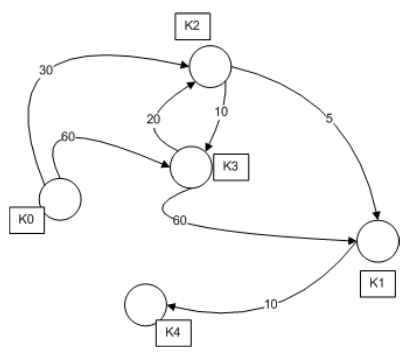
\includegraphics[scale=0.5]{figures/Algoritma_Dijkstra.PNG}
\caption{Algoritma Dijkstra}
\label{gambar2_9}
\end{figure}

Pertama-tama tentukan titik mana yang akan menjadi node awal, lalu beri bobot jarak pada node pertama ke node terdekat satu per satu, Dijkstra akan melakukan pengembangan pencarian dari satu titik ke titik lain dan ke itik selanjutnya tahap demi tahap. Inilah urutan logika dari lgoritma Dijkstra:
\begin{enumerate}
    \item Beri nilai bobot (jarak) untuk setiap titik ke titik
lainnya, lalu set nilai 0 pada node awal dan nilai tak
hingga terhadap node lain (belum terisi).
    \item Set semua node “Belum terjamah” dan set node awal
sebagai “Node keberangkatan”
    \item Dari node keberangkatan, pertimbangkan node
tetangga yang belum terjamah dan hitung jaraknya
dari titik keberangkatan. Sebagai contoh, jika titik keberangkatan K0 ke K2 memiliki bobot jarak 30 dan dari
K2 ke node K1 berjarak 5, maka jarak ke K1 melewati K2
menjadi 30+5=35. Jika jarak ini lebih kecil dari jarak
sebelumnya (yang telah terekam sebelumnya) hapus
data lama, simpan ulang data jarak dengan jarak yang
baru.
    \item Saat kita selesai mempertimbangkan setiap jarak
terhadap node tetangga, tandai node yang telah
terjamah sebagai “Node terjamah”. Node terjamah
tidak akan pernah di cek kembali, jarak yang disimpan
adalah jarak terakhir dan yang paling minimal
bobotnya.
    \item Set “Node belum terjamah” dengan jarak terkecil (dari
node keberangkatan) sebagai “Node Keberangkatan”
selanjutnya dan lanjutkan dengan kembali ke step 3.
\end{enumerate}

\section{Perhitungan Algoritma Djikstra}
\subsection{Analisis Algoritma Dijkstra}
Implementasi algoritma Dijkstra dilakukan untuk memperoleh rute terpendek yang bisa ditempuh dari suatu titik ke titik finish. Hasil yang diperoleh dari implementasi algoritma Dijkstra ini adalah rute terpendek yang terdiri dari node-node yang termasuk ke dalam solusi rute terpendek, dan total bobot minimumnya. Diskripsi matematis untuk grafik dapat diwakili G = \verb|{V. E}|, yang berarti sebuah grafik (G) didefenisikan oleh satu set simpul (Vertex = V) dan koleksi Edge (E).

Langkah-langkah algoritma Dijkstra dapat dilakukan dengan  langkah - langkah yang sudah di jelaskan pada poin \ref{Algoritma_Djikstra_Teori} bagian \ref{Algoritma_Djikstra_Teori} dan berikut tahap analisis yang dilakukan penulis dalam penerapan algoritma Dijkstra:

\begin{enumerate}
    \item Pada matriks hubungan graf table \ref{table51} sudah terdapat nilai dari setiap jalur yang akan dilewati, kemudian beri penamaan terhadap titik-titik lokasi tersebut dengan memberi label V sehingga seperti berikut :
    \par V(G)) = \verb|{V0, V1, V2, V3, V4, V5, V6, V7}|.
    
    \item Setelah titik-titik terbentuk, langkah selanjutnya adalah menghitung titik-titik yang saling berhubungan dengan cara berikut:
    \begin{enumerate}
        \item Dimulai dari menghitung G0 yaitu melihat node terdekat dari node0. Yang terdekat dari node0 adalah node1 dan node5. Node0 ke node1 memiliki jarak 543cm dan dari node0 ke node5 memiliki jarak 742cm. Nilai dari jumlah setiap jarak dimasukkan kedalam tabel V1 dan V5.

        \item Setelah itu menghitung G1 karena dari G0 nilai yang terkecil yaitu dari V1 dengan nilai 543, maka V1 terlebih dahulu yang dikerjakan atau yang dihitung jarak terhadap node yang terdekat dari V1. Selanjutnya menghitung jarak yang terhubung langsung dengan V1 yaitu V2 dan V4 dengan perhtiungan dihasilkan yaitu:
            \par G1 = V1 + (jumalah jarak node1 ke node2) = 2370
            \par G1 = V1 + (jumlah jarak node1 ke node4) = 1488
        
        \item Setelah itu menghitung G5 karena dari G1 nilai yang terkecil yaitu dari V5 dengan nilai 742, maka V5 terlebih dahulu yang dikerjakan atau yang dihitung jarak terhadap node yang terdekat dari V5. Selanjutnya menghitung jarak yang terhubung langsung dengan V5 yaitu V6 dengan perhtiungan dihasilkan yaitu:
            \par G5 = V5 + (jumalah jarak node5 ke node6) = 1520
            
        \item Setelah itu menghitung G4 karena dari G5 nilai yang terkecil yaitu dari V4 dengan nilai 1488, maka V4 terlebih dahulu yang dikerjakan atau yang dihitung jarak terhadap node yang terdekat dari V4. Selanjutnya menghitung jarak yang terhubung langsung dengan V4 yaitu V3 dengan perhtiungan dihasilkan yaitu:
            \par G4 = V4 + (jumalah jarak node4 ke node3) = 2640        

        \item Setelah itu menghitung G6 karena dari G4 nilai yang terkecil yaitu dari V6 dengan nilai 1520, maka V6 terlebih dahulu yang dikerjakan atau yang dihitung jarak terhadap node yang terdekat dari V6. Selanjutnya menghitung jarak yang terhubung langsung dengan V6 yaitu V3 dengan perhtiungan dihasilkan yaitu:
            \par G6 = V6 + (jumalah jarak node6 ke node7) = 2936

        \item Setelah itu menghitung G2 karena dari G6 nilai yang terkecil yaitu dari V2 dengan nilai 2370, maka V2 terlebih dahulu yang dikerjakan atau yang dihitung jarak terhadap node yang terdekat dari V2. Selanjutnya menghitung jarak yang terhubung langsung dengan V2 yaitu V3 dengan perhtiungan dihasilkan yaitu:
            \par G2 = V2 + (jumalah jarak node2 ke node3) = 3489
            \par Sebelumnya pada node3 sudah didapatkan jaraknya yaitu dari node 4 menuju node3 dengan nilai 2640, sedangkan nilai pada node2 menuju node3 adalah 3489. Jadi nilai yang tetap diambil adalah nilai terkceil yaitu 2640 nilai dari node4 menuju node3.

        \item Setelah itu menghitung G3 karena dari G2 nilai yang terkecil yaitu dari V3 dengan nilai 2640, maka V3 terlebih dahulu yang dikerjakan atau yang dihitung jarak terhadap node yang terdekat dari V3. Selanjutnya menghitung jarak yang terhubung langsung dengan V3 yaitu V7 dengan perhtiungan dihasilkan yaitu:
            \par G3 = V3 + (jumalah jarak node3 ke node7) = 3282
            \par Sebelumnya pada node7 sudah didapatkan jaraknya yaitu dari node 6 menuju node7 dengan nilai 2936, sedangkan nilai pada node3 menuju node7 adalah 3282. Jadi nilai yang tetap diambil adalah nilai terkceil yaitu 3282 nilai dari node6 menuju node7.
        
        \item Setelah itu G7 diturunkan saja.
        
        \item Dihasilkan table penyelesaian graf Dijkstra:
            \begin{figure}[h]
            \centering
            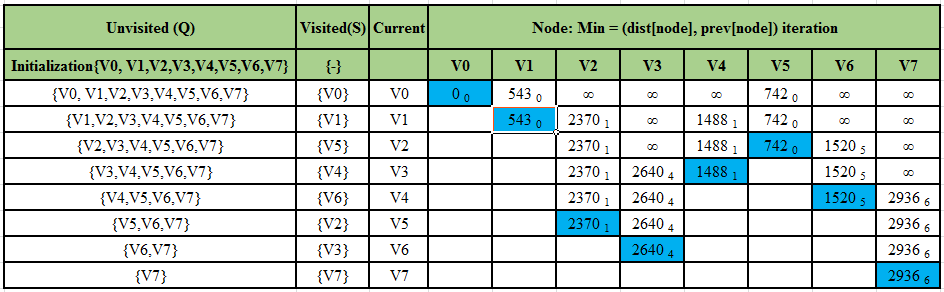
\includegraphics[scale=0.45]{figures/ALGORITMA/Matriks_Dijkstra.png}
            \caption{Matriks Dijkstra}
            \label{gambar52}
            \end{figure}
            
    \end{enumerate}
\end{enumerate}

Untuk membaca tabel perhitungan graf Dijkstra dan mengetahui lintasan mana yang terpendek yaitu:
\par 7 berasal dari node 6
\par 6 berasal dari node 5
\par 5 berasal dari node 0

Dari hasil yang didapatkan maka jalur yang terdekat yang diperoleh dari Algoritma Dijkstra adalah rute dengan titik V 0 \verb|->| 5 \verb|->| 6 \verb|->| 7 dengan jarak tempuh 2932 m. Adapun pseudocode yang akan diimplementasikan kedalam sistem berbasis web dari analisis algoritma Dijkstra adalah sebagai berikut :

\begin{lstlisting}[caption=Pseudocode Algoritma Dijkstra]
function Dijkstra(Graph, source):
      for each vertex v in Graph:                       
          dist[v] := infinity ;         
          previous[v] := undefined ;  
      end for                  
      
      dist[source] := 0 ;   
      Q := the set of all nodes in Graph ;        
      while Q is not empty:             
          u := vertex in Q with smallest distance in dist[] ;
          remove u from Q ;
          if dist[u] = infinity:
              break ;     
          end if        
          
          for each neighbor v of u:       
              alt := dist[u] + dist_between(u, v) ;
              if alt < dist[v]:  
                  dist[v] := alt ;
                  previous[v] := u ;
                  decrease-key v in Q;    
              end if
          end for
          
      end while
      
  return dist;
\end{lstlisting}
\label{PseudocodeAlgoritmaDijkstra}